\begin{frame}{Le manifeste des 343 (1971)}
  \begin{columns}
    \column{0.4\textwidth}
      \begin{center}
        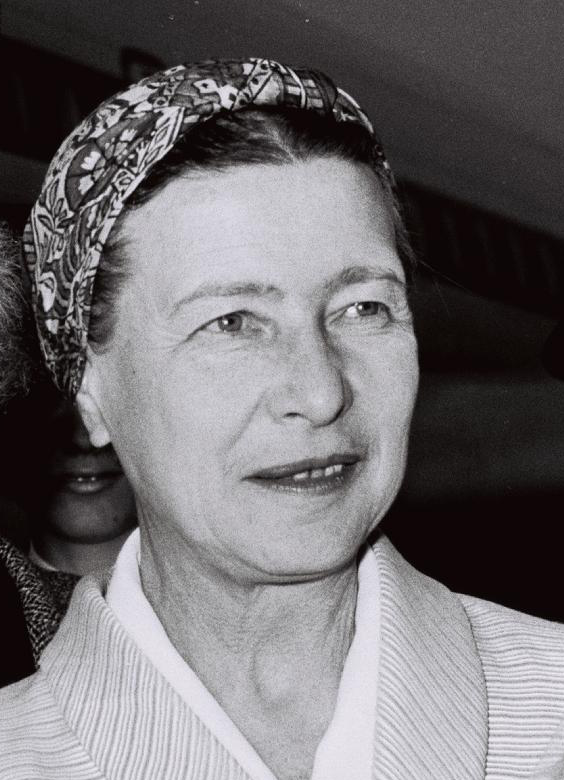
\includegraphics[scale=0.75]{beauvoir.png} \\
        Simone de Beauvoir, l'auteure
      \end{center}
    \column{0.6\textwidth}
      \only<1>{
        <<Un million de femmes se font avorter chaque année en France.
        Elles le font dans des conditions dangereuses en raison de la clandestinité à laquelle elles sont condamnées, alors que cette opération, pratiquée sous contrôle médical, est des plus simples.
        On fait le silence sur ces millions de femmes.
        Je déclare que je suis l'une d'elles. Je déclare avoir avorté.
        De même que nous réclamons le libre accès aux moyens anticonceptionnels, nous réclamons l'avortement libre.>>
      }
      \only<2>{
        Dans ce temps-là, l'avortement était illégal, et beaucoup des signataires pour cette pétition étaient des femmes célèbres (actrices, écrivaines, musiciennes).
        Pourquoi penses-tu qu'elles l'ont signé?
        Pourquoi penses-tu qu'elles ont risqué l'avortement?
        \begin{enumerate}
          \item Réfléchis et écris ta réponse.
          \item Partage ta réponse avec ton groupe et discutes-en.
        \end{enumerate}
      }
  \end{columns}
\end{frame}